\clearpage
\section{Influencia del datacenter y energía operacional estimada}
\label{sec:revision-datacenter}
El datacenter aporta 40.196,11 kWh térmicos/año en el caso base: el 47,42\,\% de la demanda de enfriamiento. Para distinguir su peso se presenta también la suma de las demás zonas. Esta exclusión es un procesamiento de las corridas existentes: mantiene sus intercambios térmicos con el datacenter y no equivale a simular la eliminación ni la reducción de su carga.
\begin{table}[H]\centering
\caption{Demanda térmica del conjunto y de las zonas distintas del datacenter}
{\small\singlespacing\renewcommand{\arraystretch}{1.2}
\begin{tabular}{lrrrr}\toprule
Caso & Total (kWh) & DC (kWh) & Sin DC (kWh) & Ahorro sin DC (\%) \\ \midrule
CB & 84.759,41 & 40.196,11 & 44.563,30 & 0,00 \\
C1 & 83.103,76 & 40.147,08 & 42.956,68 & 3,61 \\
C2 & 84.328,85 & 40.172,07 & 44.156,78 & 0,91 \\
C3 r01 & 82.748,96 & 40.125,27 & 42.623,69 & 4,35 \\
C3 r02 & 65.767,88 & 39.625,65 & 26.142,23 & 41,34 \\
\bottomrule\end{tabular}}
\fuente{Elaboración propia a partir de las corridas independientes de EnergyPlus y sus archivos de configuración.}
\end{table}

En las zonas distintas del datacenter, C3 revisión 02 reduce la demanda de 44.563,30 a 26.142,23 kWh térmicos/año (41,34\,\%). La reducción del conjunto sigue siendo 22,41\,\%. La diferencia entre ambas lecturas muestra la influencia de la carga especial en el agregado; no permite asignar ahorros a una medida individual.
\begin{figure}[H]\centering
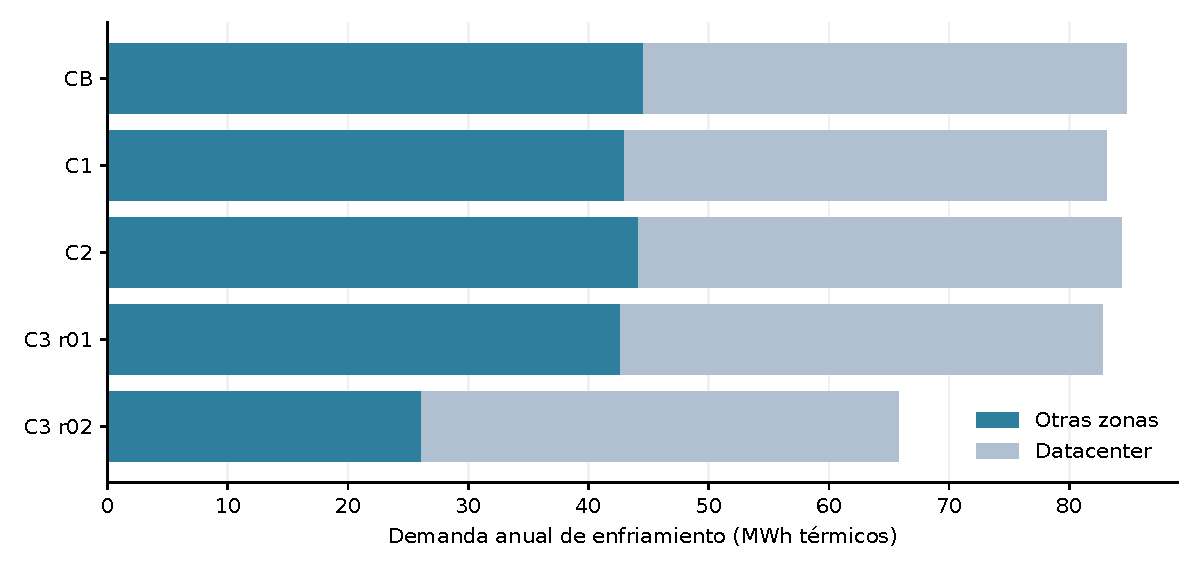
\includegraphics[width=\textwidth]{figuras/revision-datacenter.pdf}
\caption{Composición de la demanda de enfriamiento por escenario}
\fuente{Elaboración propia con registros anuales por zona. DC: datacenter. Se conserva la carga en todas las simulaciones.}
\end{figure}
\clearpage
\subsection{Estimación eléctrica y denominador de intensidad}
La electricidad de enfriamiento se reconstruye como $E_{fr}=\sum_z Q_{fr,z}/COP_z$, con las eficiencias constantes de la configuración de climatización simple. La reconstrucción del CB con la configuración conservada en C1 reproduce los 45.258,71 kWh exportados por DesignBuilder, con una diferencia inferior a 0,01 kWh. No representa el rendimiento estacional medido de equipos seleccionados. Equipos e iluminación proceden de los medidores anuales de EnergyPlus; se suman a la electricidad de enfriamiento estimada, no a la demanda térmica.
\begin{table}[H]\centering
\caption{Usos eléctricos estimados de los cinco ensayos, en kWh/año}
{\small\singlespacing\renewcommand{\arraystretch}{1.2}
\begin{tabular}{lrrrr}\toprule
Caso & Enfriamiento & Equipos & Iluminación & Total estimado \\ \midrule
CB & 45.258,71 & 39.307,57 & 13.895,39 & 98.461,67 \\
C1 & 44.413,65 & 39.307,57 & 13.895,39 & 97.616,61 \\
C2 & 45.022,61 & 39.307,57 & 13.895,39 & 98.225,57 \\
C3 r01 & 44.217,26 & 39.307,57 & 13.895,39 & 97.420,22 \\
C3 r02 & 35.553,70 & 39.307,57 & 2.258,98 & 77.120,25 \\
\bottomrule\end{tabular}}
\fuente{Elaboración propia a partir de las corridas independientes de EnergyPlus y sus archivos de configuración.}
\end{table}
La intensidad se normaliza sobre 281,63 m\textsuperscript{2}, suma de las áreas explícitas de los objetos Zone del CB excluyendo los tres atrios. Este denominador computacional común incluye circulaciones y servicios; no es superficie construida, área acondicionada certificada ni SRE Minergie. El archivo EIO infiere áreas para campos nulos y arroja 282,23 m\textsuperscript{2} sin atrios, mientras que su selección interna de área total del edificio arroja 276,04 m\textsuperscript{2}. Esas bases no se intercambian. La SRE requiere medición conforme al estándar y planos definitivos.
\begin{table}[H]\centering
\caption{Intensidad eléctrica estimada con un denominador computacional común}
{\small\singlespacing\renewcommand{\arraystretch}{1.2}
\begin{tabular}{lrr}\toprule
Caso & Área de referencia (m$^2$) & EUI (kWh/m$^2$ año) \\ \midrule
CB & 281,63 & 349,61 \\
C1 & 281,63 & 346,61 \\
C2 & 281,63 & 348,77 \\
C3 r01 & 281,63 & 345,91 \\
C3 r02 & 281,63 & 273,83 \\
\bottomrule\end{tabular}}
\fuente{Elaboración propia a partir de las corridas independientes de EnergyPlus y sus archivos de configuración.}
\end{table}
El total comprende los tres usos indicados. No se acredita un balance EDGE ni un consumo facturado; los resultados dependen de la carga continua del datacenter, los horarios y la representación idealizada de los sistemas. La reducción de iluminación incluye el efecto de los controles de luz natural configurados y requiere verificación fotométrica.